\documentclass{beamer}
\usepackage[utf8]{inputenc}

\usepackage{xcolor}
\usepackage{graphicx}
\usepackage{tikz}
\usetikzlibrary{shapes,arrows.meta,positioning,backgrounds}
\usepackage{multirow}
\usepackage{booktabs}


\definecolor{unired}{HTML}{9B0014}

\usecolortheme[named=unired]{structure}

\usetheme{Madrid}

\usepackage{tikz}
\usetikzlibrary{shapes,arrows.meta, positioning}
\usepackage{caption}

% Blocchi senza barra nera sul titolo
\setbeamertemplate{blocks}[rounded][shadow=false]
\setbeamercolor{block title}{fg=white,bg=unired} % titolo bianco su sfondo rosso
\setbeamercolor{block body}{fg=black,bg=unired!10} % corpo testo su sfondo rosso chiaro


\title[Mindfulness e marcatori dello stress]{Mindfulness e marcatori dello stress:\\uno studio di meta-analisi}

\author{Federica Belardinelli}

\date[16 settembre 2025]{}

\begin{document}

\begin{frame}[label = cover]
    \centering

    % Titolo e sottotitolo
    \begin{beamercolorbox}[rounded = true, shadow = true, center, wd = \textwidth]{title}
        \usebeamerfont{title}
        {\color{white}\inserttitle}\\[0.2cm]
        \usebeamerfont{subtitle}{\normalsize Discussione relazione finale}
    \end{beamercolorbox}

    \vspace{0.75em}

    % Immagine
    \includegraphics[width = 0.25\textwidth]{logo.png}

    % Autore e informazioni accademiche
    \vspace{0.75em}

    {\large\textbf{Federica Belardinelli}}\\[0.5em]
    {Corso di Laurea Triennale in Statistica per le Tecnologie e le Scienze}\\[1em]

    % Colonna per il relatore
    \begin{columns}
        \column{0.45\textwidth}
        \raggedright
        \textbf{Relatore}\\
        Prof. Annamaria Guolo

        \column{0.45\textwidth}
        \raggedleft
    \end{columns}

    \vfill

    {\small A.A. 2024/2025}
\end{frame}

\begin{frame}{Stress e salute}
  Lo stress è un \textbf{fattore di rischio} psicologico e fisiologico.

  \vspace{1em}

  \begin{itemize}
    \item \textbf{Psicologico}: favorisce ansia e depressione
    \item \textbf{Fisiologico}: attiva il sistema nervoso simpatico (SNS) 
          e l’asse ipotalamo--ipofisi--surrene (HPA).
  \end{itemize}
\end{frame}

\begin{frame}{Mindfulness}
  \begin{block}{Definizione di mindfulness}
    Insieme di \textbf{pratiche mentali} per migliorare le capacità psicologiche dell'individuo, come l'autoregolamentazione emotiva e attenzionale.
  \end{block}
  \begin{itemize}
    \item \textbf{FA}: attenzione focalizzata (es.\ respiro).
    \item \textbf{OM}: monitoraggio aperto di pensieri/sensazioni senza giudizio.
    \item \textbf{AST}: trascendimento spontaneo dell'attività mentale.
  \end{itemize}
\end{frame}

\begin{frame}{Studio di riferimento e focus della tesi}
  \textbf{Studio di riferimento} \\
  Pascoe et al.\ (2017): meta-analisi di 45 RCT sui marcatori dello stress.

  \vspace{1em}

  \textbf{Focus della tesi} \\
  Analisi approfondita di tre indicatori principali:
  \begin{itemize}
    \item Cortisolo
    \item Pressione arteriosa sistolica (SBP)
    \item Pressione arteriosa diastolica (DBP)
  \end{itemize}
\end{frame}

\begin{frame}{Cos’è la meta-analisi}
  \begin{block}{Definizione}
    La \textbf{meta-analisi}, introdotta da \textbf{Gene V. Glass} negli anni ’70, 
    viene definita come \textbf{“analisi delle analisi”}.
  \end{block}

  \vspace{0.8em}

  \begin{itemize}
    \item Combina i risultati di studi indipendenti già condotti.
    \item Fornisce una stima unica, più precisa e affidabile.
  \end{itemize}
\end{frame}

\begin{frame}{Modelli a effetti fissi e a effetti casuali}
  \begin{columns}[T]
    % --- Effetti fissi ---
    \begin{column}{0.48\textwidth}
      \centering
      \textbf{Effetti fissi (FE)} \\[0.1em]
      \[
        Y_i = \beta + \varepsilon_i, 
        \quad \varepsilon_i \sim \mathcal{N}(0,\sigma_i^2)
      \]
      \vspace{0.6em}
      \footnotesize Tutti gli studi stimano la stessa vera misura d’effetto.
    \end{column}

    % --- Effetti casuali ---
    \begin{column}{0.48\textwidth}
      \centering
      \textbf{Effetti casuali (RE)} \\[0.1em]
      \[
        Y_i = \beta_i + \varepsilon_i, \quad 
        \beta_i = \beta + \eta_i
      \]
      \[
        \varepsilon_i \sim \mathcal{N}(0,\sigma_i^2), 
        \quad \eta_i \sim \mathcal{N}(0,\tau^2)
      \]
      \vspace{0.6em}
      \footnotesize La vera misura d’effetto può variare \\tra studi (varianza $\tau^2$).
    \end{column}
  \end{columns}
\end{frame}

\begin{frame}{Metodi di stima}
  \textbf{Contesto:} si presentano i metodi di stima utilizzati nella tesi. Sono tutti relativi al \textbf{modello a effetti casuali}, 
  poiché nella pratica è sempre presente eterogeneità tra studi.  

  \vspace{1em}

  Obiettivi principali:
  \begin{itemize}
    \item stimare l’effetto medio $\beta$
    \item stimare la varianza tra studi $\tau^2$
  \end{itemize}
\end{frame}

\begin{frame}{Metodo tradizionale: DerSimonian e Laird}
  \[
    \hat{\beta}_{DL} = 
    \frac{\sum_{i=1}^n \hat{w}_i Y_i}{\sum_{i=1}^n \hat{w}_i},
    \qquad 
    \hat{w}_i = \frac{1}{\sigma_i^2+\hat{\tau}^2}
  \]

  \vspace{1em}

  \[
    \hat{\tau}^2_{DL} = 
    \max\!\left\{0,\;
    \frac{Q - (n-1)}{\sum_{i=1}^n w_i - \sum_{i=1}^n w_i^2/\sum_{i=1}^n w_i}
    \right\},
    \qquad
    w_i = \frac{1}{\sigma_i^2}
  \]

  \vspace{1em}

  \textbf{Nota:} semplice e veloce, ma presenta limitazioni.
\end{frame}

\begin{frame}<1-3>{Metodi avanzati}

\centering
\begin{tikzpicture}[x=\textwidth,y=1cm]
  % Coordinate estremi con margini
  \coordinate (A) at (0.1,0);
  \coordinate (B) at (0.9,0);

  % Linea di collegamento (dietro)
  \draw[black!25, line width=1.2pt, line cap=round] (A) -- (B);

  % Pallini base
  \node[circle, draw=black, fill=white, minimum size=9mm, very thick] (d1) at (0.1,0) {1};
  \node[circle, draw=black, fill=white, minimum size=9mm, very thick] (d2) at (0.5,0) {2};
  \node[circle, draw=black, fill=white, minimum size=9mm, very thick] (d3) at (0.9,0) {3};

  % Pallino attivo
  \only<1>{\node[circle, draw=unired, fill=unired, text=white, minimum size=9mm, very thick] at (d1) {1};}
  \only<2>{\node[circle, draw=unired, fill=unired, text=white, minimum size=9mm, very thick] at (d2) {2};}
  \only<3>{\node[circle, draw=unired, fill=unired, text=white, minimum size=9mm, very thick] at (d3) {3};}

  % Etichette sotto
  \node[font=\footnotesize, anchor=north] at (d1.south) {\textbf{Massima verosimiglianza}};
  \node[font=\footnotesize, anchor=north] at (d2.south) {\textbf{Massima verosimiglianza ristretta}};
  \node[font=\footnotesize, anchor=north] at (d3.south) {\textbf{Skovgaard}};
\end{tikzpicture}

\vspace{1em}
\raggedright

% --- Contenuto che cambia ---
\only<1>{
  Tiene conto dell’incertezza nella stima dell’eterogeneità racchiusa dal parametro $\tau^2$.

  \begin{equation*}
    \ell(\beta, \tau^2; y_1,\dots,y_n) = -\frac{1}{2}\sum_{i=1}^{n}\log(\tau^2+\sigma^2_i)
    -\frac{1}{2}\sum_{i=1}^{n}\frac{(y_i - \beta)^2}{\tau^2 + \sigma^2_i}
  \end{equation*}

}

\only<2>{
  Riduce il \textit{bias negativo} associato alla stima di massima verosimiglianza di $\tau^2$ ottenuta con la massima verosimiglianza.

  \begin{equation*}
    \ell_{REML}(\tau^2) = -\frac{1}{2}\sum_{i=1}^{n}\log(\sigma^2_i + \tau^2) - \frac{1}{2}\sum_{i=1}^{n}\log\frac{1}{(\sigma^2_i+\tau^2)} - \frac{1}{2}\sum_{i=1}^{n}\frac{r_i^2}{\sigma^2_i+\tau^2}
  \end{equation*}

}

\only<3>{
  Si tratta di una correzione applicabile alla radice con segno del log-rapporto di verosimiglianza $r_\text{P}(\beta)$. Si rivela utile quando il numero di studi è ridotto.

  \begin{equation*}
    \bar{r}_\text{P}(\beta) = r_\text{P}(\beta) + \frac{1}{r_\text{P}(\beta)}\log\frac{\bar{u}(\beta)}{r_\text{P}(\beta)}
  \end{equation*}

}
\end{frame}

\begin{frame}{Eterogeneità tra studi}

\textbf{Strumenti principali:}

\begin{enumerate}
  \item \textbf{Test $Q$ di Cochran}
  
  \[
    Q = \sum_{i=1}^n (Y_i - \hat{\beta}_{FE})^2w_i, 
    \qquad \hat{\beta}_{FE} = \frac{\sum_{i=1}^nw_iY_i}{\sum_{i=1}^nw_i}
  \]
  
  \item \textbf{Indice $I^2$}
  
  \[
    I^2 = \max\!\left(0,\,\frac{Q-(n-1)}{Q}\right)\times 100\%
  \]
  
  \item \textbf{Indice $H^2$}
  
  \[
    H^2 = \frac{Q}{n-1}
  \]
  
\end{enumerate}

\end{frame}

\begin{frame}{Meta-regressione a effetti casuali}

\textbf{Modello:}
\[
  Y_i = \beta_0 + \beta_1 x_{i1} + \dots + \beta_p x_{ip} + u_i + \varepsilon_i,
  \quad \varepsilon_i \sim N(0,\sigma_i^2),\quad
  u_i \sim N(0,\tau^2)
\]

\textbf{Test $Q_M$:} per verificare l'ipotesi secondo cui i moderatori non spiegano eterogeneità.

\[
  Q_M = \hat{\boldsymbol{\beta}}^T Var(\hat{\boldsymbol{\beta}})^{-1}
        \hat{\boldsymbol{\beta}}
\]

\end{frame}

\begin{frame}{Meta-analisi multivariata}

\textbf{Modello:}
\[
  \mathbf{Y}_i \sim \mathcal{N}_m(\boldsymbol{\beta},\; \Sigma_i + \Psi)
\]

\vspace{0.5em}

\textbf{Vantaggi:}
\begin{itemize}
  \item Tiene conto delle \textbf{correlazioni} tra effetti.
  \item Fornisce stime più \textbf{efficienti} e inferenza più \textbf{corretta}.
\end{itemize}

\end{frame}

\begin{frame}{Impostazione delle analisi}

\begin{itemize}
  \item Gli outcome (cortisolo, SBP, DBP) sono espressi come:
    \begin{itemize}
      \item \textbf{Differenza media (MD)} tra gruppo mindfulness e controllo,
      \item \textbf{Differenza media standardizzata} \textbf{SMD} se le scale di misura differiscono.
    \end{itemize}

  \vspace{0.6em}

  \item Le analisi sono condotte con \textbf{modelli a effetti casuali}.

  \vspace{0.6em}

  \item Livello di significatività adottato: \textbf{$\alpha = 0.05$}.
\end{itemize}

\end{frame}


% =========================
% SEZIONE: CORTISOLO
% =========================
\section{Cortisolo}

\begin{frame}{Cortisolo — forest plot}
  \centering
  \includegraphics[width=0.65\textwidth]{forest_cortisol.png}
\end{frame}

% --- Slide 2: Confronto metodi ---
\begin{frame}{Cortisolo — modello a effetti casuali}
  \begin{table}[H]
  \centering
  \begin{tabular}{lcccccc}
  \hline
  \textbf{Metodo} & $\hat{\beta}$ & s.e. & $z$ & $p$-value & ci.lb & ci.ub \\
  \hline
  \textbf{DL} & $-0.412$ & $0.156$ & $-2.650$ & $0.008$ & $-0.718$ & $-0.107$ \\
  \textbf{ML} & $-0.413$ & $0.155$ & $-2.657$ & $0.008$ & $-0.717$ & $-0.108$ \\
  \textbf{REML} & $-0.412$ & $0.157$ & $-2.618$ & $0.009$ & $-0.720$ & $-0.103$ \\
  \hline
  \end{tabular}
  \caption{Stima puntuale dell’effetto medio, deviazione standard, valore $z$ della statistica test alla Wald, $p$-value, estremo inferiore ed estremo superiore dell'intervallo di confidenza del modello a effetti casuali adattato con i metodi DL, ML, REML.}
  \end{table}

  \vspace{1em}
  \textbf{Skovgaard:} $-1.824$, \quad $p=0.068$.
\end{frame}

% --- Slide 3: Eterogeneità ---
\begin{frame}{Cortisolo — eterogeneità}
  \begin{table}[H]
  \centering
  \begin{tabular}{lccccc}
  \hline
  \textbf{Metodo} & $I^2$ & $H^2$ & $\hat\tau^2$ & ci.lb & ci.ub \\
  \hline
  \textbf{DL} & $0.38\%$ & $1.00$ & $\approx 0$ & $0.000$ & $0.792$ \\
  \textbf{ML} & $0.00\%$ & $1.00$ & $\approx 0$ & $0.000$ & $0.361$ \\
  \textbf{REML} & $2.15\%$ & $1.02$ & $\approx 0$ & $0.000$ & $0.571$ \\
  \hline
  \end{tabular}
  \caption{Statistiche di eterogeneità $I^2$ e $H^2$, stima puntuale di $\tau^2$, estremo inferiore ed estremo superiore dell'intervallo di confidenza per $\tau^2$ calcolati con i metodi DL, ML e REML.}
  \end{table}

  \vspace{1em}
  \textbf{Test $Q$}: $5.019$, \quad $p=0.414$.
\end{frame}

% --- Slide 4: Meta-regressione e scelta del modello ---
\begin{frame}{Cortisolo — meta-regressione e scelta del modello finale}

\textbf{Meta-regressione (modello a effetti casuali)}  
\begin{itemize}
  \item Moderatore: tipologia di mindfulness (FA, AST).  
  \item Test alla Wald: $-1.508$, \quad $p = 0.132$.  
  \item Risultati identici con DL, ML, REML.  
  \item \textbf{Skovgaard:} $-1.323$, \quad $p=0.186$.  
\end{itemize}

\vspace{1em}

\textbf{Scelta del modello e del metodo}  
\begin{itemize}
  \item In tutti i casi si adotta il modello a \textbf{effetti casuali}.  
  \item Confronto \textbf{AIC}: ML = $8.755$, \quad REML = $8.848$.  
  \item Metodo finale: \textbf{ML} (AIC più basso).  
\end{itemize}

\end{frame}

% --- Slide 5: diagnostiche ---
\begin{frame}{Cortisolo — analisi diagnostiche}
  \begin{figure}
    \centering
    \begin{minipage}{0.45\textwidth}
      \centering
      \includegraphics[width=\textwidth]{influence_cortisol.png}
      \caption{Grafico dei punti influenti.}
    \end{minipage}\hfill
    \begin{minipage}{0.45\textwidth}
      \centering
      \includegraphics[width=\textwidth]{baujat_cortisol.png}
      \caption{Baujat plot.}
    \end{minipage}
  \end{figure}
\end{frame}

% =========================
% SEZIONE: SBP
% =========================
\section{SBP}

\begin{frame}{SBP — forest plot}
  \centering
  \includegraphics[width=0.65\textwidth]{forest_rsbp.png}
\end{frame}

% --- Slide 2: Confronto metodi ---
\begin{frame}{SBP — modello a effetti casuali}
  \begin{table}[H]
  \centering
  \begin{tabular}{lcccccc}
  \hline
  \textbf{Metodo} & $\hat{\beta}$ & s.e. & $z$ & $p$-value & ci.lb & ci.ub \\
  \hline
  \textbf{DL} & $-5.372$ & $1.467$ & $-3.662$ & $<0.001$ & $-8.247$ & $-2.497$ \\
  \textbf{ML} & $-4.903$ & $1.076$ & $-4.555$ & $<0.001$ & $-7.012$ & $-2.793$ \\
  \textbf{REML} & $-5.181$ & $1.291$ & $-4.013$ & $<0.001$ & $-7.711$ & $-2.651$ \\
  \hline
  \end{tabular}
  \caption{Stima puntuale dell’effetto medio, deviazione standard, valore $z$ della statistica test alla Wald, $p$-value, estremo inferiore ed estremo superiore dell'intervallo di confidenza del modello a effetti casuali adattato con i metodi DL, ML, REML.}
  \end{table}

  \vspace{1em}
  \textbf{Skovgaard:} $-2.560$, \quad $p=0.011$.
\end{frame}

% --- Slide 3: Eterogeneità ---
\begin{frame}{SBP — eterogeneità}
  \begin{table}[H]
  \centering
  \begin{tabular}{lccccc}
  \hline
  \textbf{Metodo} & $I^2$ & $H^2$ & $\hat\tau^2$ & ci.lb & ci.ub \\
  \hline
  \textbf{DL} & $34.85\%$ & $1.53$ & $7.933$ & $0.000$ & $>100.000$ \\
  \textbf{ML} & $0.00\%$ & $1.00$ & $\approx 0$ & $0.000$ & $37.693$ \\
  \textbf{REML} & $20.37\%$ & $1.26$ & $3.535$ & $0.000$ & $55.642$ \\
  \hline
  \end{tabular}
  \caption{Statistiche di eterogeneità $I^2$ e $H^2$, stima puntuale di $\tau^2$, estremo inferiore ed estremo superiore dell'intervallo di confidenza per $\tau^2$ calcolati con i metodi DL, ML e REML.}
  \end{table}

  \vspace{1em}
  \textbf{Test $Q$}: $15.349$, \quad $p=0.120$.
\end{frame}

% --- Slide 4: Meta-regressione e scelta del modello ---
\begin{frame}{SBP — meta-regressione e scelta del modello finale}

\textbf{Meta-regressione (modello a effetti casuali)}  
\begin{itemize}
  \item Moderatore: tipologia di mindfulness (FA, OM, AST).  
  \item Risultati del test $Q_M$ per diversi metodi:
\end{itemize}

\begin{table}[H]
  \centering
  \begin{tabular}{lcc}
  \hline
  \textbf{Metodo} & $Q_M$ & $p$-value \\
  \hline
  \textbf{DL} & $2.636$ & $0.268$ \\
  \textbf{ML} & $4.148$ & $0.126$ \\
  \textbf{REML} & $4.148$ & $0.126$ \\
  \hline
  \end{tabular}
  \caption{Test $Q_M$ e $p$-value per i metodi DL, ML, REML.}
\end{table}

\textbf{Scelta del modello e del metodo}  
\begin{itemize}
  \item In tutti i casi si adotta il modello a \textbf{effetti casuali}.  
  \item Confronto AIC: ML = $72.122$, REML = $67.570$.  
  \item Metodo finale: \textbf{REML} (AIC più basso).  
\end{itemize}

\end{frame}

% --- Slide 5: diagnostiche ---
\begin{frame}{SBP — analisi diagnostiche}
  \begin{figure}
    \centering
    \begin{minipage}{0.45\textwidth}
      \centering
      \includegraphics[width=\textwidth]{influence_rsbp.png}
      \caption{Grafico dei punti influenti.}
    \end{minipage}\hfill
    \begin{minipage}{0.45\textwidth}
      \centering
      \includegraphics[width=\textwidth]{baujat_rsbp.png}
      \caption{Baujat plot.}
    \end{minipage}
  \end{figure}
\end{frame}

% =========================
% SEZIONE: DBP
% =========================
\section{DBP}

\begin{frame}{DBP — forest plot}
  \centering
  \includegraphics[width=0.65\textwidth]{forest_rdbp.png}
\end{frame}

% --- Slide 2: Confronto metodi ---
\begin{frame}{DBP — modello a effetti casuali}
  \begin{table}[H]
  \centering
  \begin{tabular}{lcccccc}
  \hline
  \textbf{Metodo} & $\hat{\beta}$ & s.e. & $z$ & $p$-value & ci.lb & ci.ub \\
  \hline
  \textbf{DL} & $-2.958$ & $1.076$ & $-2.748$ & $0.006$ & $-5.068$ & $-0.849$ \\
  \textbf{ML} & $-2.946$ & $1.061$ & $-2.778$ & $0.005$ & $-5.025$ & $-0.867$ \\
  \textbf{REML} & $-2.989$ & $1.121$ & $-2.666$ & $0.008$ & $-5.187$ & $-0.792$ \\
  \hline
  \end{tabular}
  \caption{Stima puntuale dell’effetto medio, deviazione standard, valore $z$ della statistica test alla Wald, $p$-value, estremo inferiore ed estremo superiore dell'intervallo di confidenza del modello a effetti casuali adattato con i metodi DL, ML, REML.}
  \end{table}

  \vspace{1em}
  \textbf{Skovgaard:} $-2.328$, \quad $p=0.020$.
\end{frame}

% --- Slide 3: Eterogeneità ---
\begin{frame}{DBP — eterogeneità}
  \begin{table}[H]
  \centering
  \begin{tabular}{lccccc}
  \hline
  \textbf{Metodo} & $I^2$ & $H^2$ & $\hat\tau^2$ & ci.lb & ci.ub \\
  \hline
  \textbf{DL} & $57.11\%$ & $2.33$ & $6.662$ & $0.697$ & $33.997$ \\
  \textbf{ML} & $55.85\%$ & $2.27$ & $6.329$ & $0.143$ & $26.790$ \\
  \textbf{REML} & $60.47\%$ & $2.53$ & $7.653$ & $0.579$ & $32.384$ \\
  \hline
  \end{tabular}
  \caption{Statistiche di eterogeneità $I^2$ e $H^2$, stima puntuale di $\tau^2$, estremo inferiore ed estremo superiore dell'intervallo di confidenza per $\tau^2$ calcolati con i metodi DL, ML e REML.}
  \end{table}

  \vspace{1em}
  \textbf{Test $Q$}: $23.316$, \quad $p=0.010$.
\end{frame}

% --- Slide 4: Meta-regressione e scelta del modello ---
\begin{frame}{DBP — meta-regressione e scelta del modello finale}

\textbf{Meta-regressione (modello a effetti casuali)}  
\begin{itemize}
  \item Moderatore: tipologia di mindfulness (FA, OM, AST).  
  \item Risultati del test $Q_M$ per diversi metodi:
\end{itemize}

\begin{table}[H]
  \centering
  \begin{tabular}{lcc}
  \hline
  \textbf{Metodo} & $Q_M$ & $p$-value \\
  \hline
  \textbf{DL} & $3.567$ & $0.168$ \\
  \textbf{ML} & $5.627$ & $0.060$ \\
  \textbf{REML} & $3.320$ & $0.190$ \\
  \hline
  \end{tabular}
  \caption{Test $Q_M$ e $p$-value per i metodi DL, ML, REML.}
\end{table}

\textbf{Scelta del modello e del metodo}  
\begin{itemize}
  \item In tutti i casi si adotta il modello a \textbf{effetti casuali}.  
  \item Confronto AIC: ML = $63.230$, REML = $58.821$.  
  \item Metodo finale: \textbf{REML} (AIC più basso).  
\end{itemize}

\end{frame}

% --- Slide 5: diagnostiche ---
\begin{frame}{DBP — analisi diagnostiche}
  \begin{figure}
    \centering
    \begin{minipage}{0.45\textwidth}
      \centering
      \includegraphics[width=\textwidth]{influence_rdbp.png}
      \caption{Grafico dei punti influenti.}
    \end{minipage}\hfill
    \begin{minipage}{0.45\textwidth}
      \centering
      \includegraphics[width=\textwidth]{baujat_rdbp.png}
      \caption{Baujat plot.}
    \end{minipage}
  \end{figure}
\end{frame}

\begin{frame}{Meta-analisi multivariata}
\begin{itemize}
  \item Analisi congiunta di \textbf{SBP} e \textbf{DBP}.
  \item Modello a \textbf{effetti casuali multivariato}, stimato con ML e REML.
  
  \begin{table}[H]
  \scriptsize
  \centering
  \begin{tabular}{lccccccc}
  \hline
  Metodo & Variabile & $\hat{\beta}$ & s.e. & $z$ & $p$-value & ci.lb & ci.ub \\
  \toprule
  \multirow{2}{*}{ML} 
    & $SBP$ & $-6.919$ & $2.060$ & $-3.359$ & $<0.001$ & $-10.956$ & $-2.882$ \\
    & $DBP$ & $-3.343$ & $1.411$ & $-2.369$ & $0.018$ & $-6.110$ & $-0.577$ \\
  \midrule
  \multirow{2}{*}{REML} 
    & $SBP$ & $-6.912$ & $2.155$ & $-3.208$ & $0.001$ & $-11.135$ & $-2.689$ \\
    & $DBP$ & $-3.358$ & $1.451$ & $-2.314$ & $0.021$ & $-6.202$ & $-0.514$ \\
  \bottomrule
  \end{tabular}
  \caption{Stime puntuali degli effetti medi relativi alle variabili $SBP$ e $DBP$, deviazioni standard, valore $z$ della statistica test alla Wald, $p$-value, estremo inferiore ed estremo superiore dell'intervallo di confidenza  nel modello a effetti casuali adattato con i metodi ML e REML.}
  \end{table}

  \item Risultati coerenti con gli univariati.
\end{itemize}
\end{frame}

\begin{frame}{Eterogeneità (multivariata)}
\begin{itemize}
  \item \textbf{Indice $I^2$} (identico con ML, REML): $82.1\%$.
  \item \textbf{Test $Q$}: $111.863$, \quad $p < 0.001$.
\end{itemize}
\end{frame}

\begin{frame}{Meta-regressione multivariata e scelta del modello finale}
\textbf{Meta-regressione multivariata (modello a effetti casuali)} 
\begin{itemize}
  \item Moderatore: tipologia di mindfulness (FA, OM, AST).
  \item \textbf{ML:} LR test $= 3.475$, \quad $p = 0.482$.
  \item \textbf{REML:} Wald $= 3.300$, \quad $p = 0.510$.
\end{itemize}

\vspace{1em}

\textbf{Scelta del modello e del metodo}
\begin{itemize}
  \item In tutti i casi si adotta il modello a \textbf{effetti casuali}.
  \item Confronto AIC: ML = $140.882$, REML = $122.285$.
  \item Metodo finale: \textbf{REML} (AIC più basso).
\end{itemize}
\end{frame}

\begin{frame}{Possibili sviluppi futuri}
\begin{itemize}
  \item Ampliare il numero di studi disponibili nelle meta-analisi.  
  \item Sviluppare e perfezionare gli approcci \textbf{multivariati}.
  \item Estendere le analisi includendo la verifica del \textbf{publication bias}.  
\end{itemize}
\end{frame}

\begin{frame}{Riferimenti bibliografici}
\scriptsize
\begin{columns}[t]
  \begin{column}{0.48\textwidth}
    \begin{thebibliography}{9}

    \bibitem{Baujat2002}
    Baujat, B., Mahé, C., Pignon, J. P. \& Hill, C. (2002).  
    A graphical method for exploring heterogeneity in meta-analyses: application to a meta-analysis of 65 trials.  
    \emph{Statistics in Medicine}, 21(18), 2641–2652.

    \bibitem{Creswell2017}
    Creswell, J. D. (2017).  
    Mindfulness Interventions.  
    \emph{Annual Review of Psychology}, 68, 491–516.

    \bibitem{DerSimonian1986}
    DerSimonian, R. \& Laird, N. (1986).  
    Meta-analysis in clinical trials.  
    \emph{Controlled Clinical Trials}, 7(3), 177–188.

    \bibitem{Glass1976}
    Glass, G. V. (1976).  
    Primary, Secondary, and Meta-Analysis of Research.  
    \emph{Educational Researcher}, 5(10), 3–8.

    \bibitem{GuoloVarin2017}
    Guolo, A. \& Varin, C. (2017).  
    Random-effects meta-analysis: The number of studies matters.  
    \emph{Statistical Methods in Medical Research}, 26(3), 1500–1518.

    \end{thebibliography}
  \end{column}

  \begin{column}{0.48\textwidth}
    \begin{thebibliography}{9}

    \bibitem{Hartung2001}
    Hartung, J. \& Knapp, G. (2001).  
    A refined method for the meta-analysis of controlled clinical trials with binary outcome.  
    \emph{Statistics in Medicine}, 20(24), 3875–3889.

    \bibitem{Higgins2002}
    Higgins, J. P. T. \& Thompson, S. G. (2002).  
    Quantifying heterogeneity in a meta-analysis.  
    \emph{Statistics in Medicine}, 21(11), 1539–1558.

    \bibitem{Pascoe2017}
    Pascoe, M. C., Thompson, D. R., Jenkins, Z. M. \& Ski, C. F. (2017).  
    Mindfulness mediates the physiological markers of stress: Systematic review and meta-analysis.  
    \emph{Journal of Psychiatric Research}, 95, 156–178.

    \bibitem{Tang2015}
    Tang, Y. Y., Hölzel, B. K. \& Posner, M. I. (2015).  
    The neuroscience of mindfulness meditation.  
    \emph{Nature Reviews Neuroscience}, 16(4), 213–225.

    \end{thebibliography}
  \end{column}
\end{columns}
\end{frame}

\begin{frame}
  \centering
  \vfill
  {\Huge\textbf{Grazie per l’attenzione!}} \\[1em]
  \rule{0.5\textwidth}{0.6pt}
  \vfill
\end{frame}












\end{document}
